\iffalse
\section{Todo notes}

Equations of state
\begin{itemize}
    \item Bag model \cite[eq. 7.33]{lecture_notes}
    \item Assumptions on speed of sound and constant parameters
    \item Giese's paper \cite{giese_2020}
    \item Enqvist, old paper \cite{enqvist_nucleation_1992}
\end{itemize}

Employment?
- "things that need to be done"
-> suitable for public dissemination
- write some short description,
    - ArXiv paper

2 papers by Giese, second one is more complete
Paper 1 \cite{giese_2020}
Paper 2 \cite{giese_2021}

TODO: understand these
\begin{itemize}
    \item Relativistic hydrodynamics from the review article (aka. lecture notes) \cite{lecture_notes}
    \item Reviews from other people (not just Hindmarsh)
    \item Article by Mazumdar \& White, especially section 7: relativistic combustion \cite{mazumdar_review_2019}
    \item The sound shell model paper
    \item Really understand what's going on! Compute with pen \& paper etc.
    \item Relativistic hydrodynamics
    \begin{itemize}
        \item The book by Luciano Rezzolla \& Olindo Zanotti \cite{rezzolla_relativistic_2013}
        \item Read the part I (some 300 pages at first)
        \item Contains more than necessary for the thesis
    \end{itemize}
    \item The phase transition section should have plenty of content before Christmas
    \item Enqvist's paper
    \begin{itemize}
        \item Good background: connects the equations of state to particle physics
        \item -> What kinds of equations of state would a particle theory produce
        \item Assumes ultrarelativisticity, which is no longer necessary due to the improvement of computational tools
    \end{itemize}
    \item Ultimately the equation of state can be derived from the "Thermal effective potential".
    \item Chemical potential is zero, as there is no conserved particle number.
    \item J-function, fB, lecture eq. 2.19 etc.
    \begin{itemize}
        \item These will be our first equation of state.
    \end{itemize}
\end{itemize}

"My job is to give the GWs the right energy-momentum tensor"

Electroweak symmetry breaking at
First-order phase transition
-> bubbles just below the critical temperature
-> gravitational waves

Standard model has a crossover, but many extensions first-order.

Matter-antimatter asymmetry -> net baryon number
(But isn't B an accidental symmetry, whereas B-L is a fundamental one?
How does this correspond to the neutrino content of the universe?)
\cite{lecture_notes}

The gravitational wave spectrum can be calculated from a few thermodynamic properties of ultrarelativistic matter, which can be computed from quantum field theory.
These parameters can be measured by LISA.
\fi

The early universe has undergone multiple phase transitions.
Among the most notable of these is the electroweak symmetry breaking, also known as the Higgs transition, at around $10^{-11}$ s and $100$ -- $1000$ GeV,
when the electromagnetic interaction separated from the weak interaction and the Higgs mechanism turned on,
giving the gauge bosons their rest masses.
Another notable phase transition is the QCD phase transition at around $10^{-5}$ s and $200$ MeV,
when the quarks of the quark-gluon plasma of the early universe became bound into hadrons.
In the Standard Model these are both second-order phase transitions, also known as crossovers.
\cites{lecture_notes}{aoki_order_2006}

The electroweak symmetry breaking is of particular interest,
as the transition is of first order in various extensions of the Standard Model.
A first-order phase transition results in a departure from thermal equilibrium,
which is a requirement for the formation of matter-antimatter asymmetry.
This generation of net baryon number is known as baryogenesis.
\cite{lecture_notes}

The theory of first-order phase transitions in the early universe is based on relativistic hydrodynamics.
The following section \ref{rel_hydro} starts from the energy-momentum tensor of general relativity and derives the equations that
govern the evolution of the fluid: the relativistic Euler equation, the energy-conservation equation and the wave equation.
Section \ref{relativistic_combustion} proceeds to the process of relativistic combustion and derives the bubble wall junction conditions
that define the behaviour of the fluid velocities and thermodynamic quantities at the bubble wall.
It then defines various equations and quantities that will be of use in the simulations,
including the transition strength $\alpha$ and a ordinary differential equation group that determines the fluid velocity profile of the bubble.
Section \ref{solution_types} investigates the different types of solutions that these equations allow,
and the speed limits associated with these solutions.
Section \ref{general_eq} derives the general equation of state,
and section \ref{bag_model} introduces its simplest implementation, the bag model.
Section \ref{const_cs} extends the bag model to having different sound speeds in each phase,
resulting in the constant sound speed model.
Finally section \ref{energy_redistribution} investigates how the phase transition affects the distribution of energy between the field and the kinetic and thermal energies of the fluid.


\section{Relativistic hydrodynamics}
\label{rel_hydro}
% Statistical mechanics \cite{huang_statistical_1987}
% \cite{schroeder_thermal_2000}
% \cite[ch. 4]{lecture_notes}
% According to Hindmarsh it's OK to have references on the level of individual chapters and equations.

Our system of interest is an ultrarelativistic plasma.
This means, that the energy of the particles is much higher than their rest mass.
Therefore there is sufficient energy for new particles to be created,
and similarly existing particles will annihilate all the time.
Treating this kind of a system as a classical fluid is not sufficient,
and we need the mathematical machinery of general relativity.
It should be noted that the Einstein notation will be used for the indices throughout the thesis.
Greek indices are used for four-vectors and latin indices for three-vectors.
% The Einstein notation is absolute basics for theoretical physicists, but unfortunately the study programme of many of my applied/technical physicists friends doesn't involve it, so I'm mentioning it explicitly here so that they can google it.

In general relativity the matter and energy content of space are described by the energy-momentum tensor $T_{\mu \nu}$, also known as the stress-energy tensor.
\iffalse
Without loss of generality it can be decomposed as
\begin{equation}
T_{\mu \nu} = e u_\mu u_\nu + p h_{\mu \nu} + 2 q_{(\mu} u_{\beta)} + \Pi_{\mu \mu},
\end{equation}
where $h_{\mu \nu} = g_{\mu \nu} + u_\alpha u_\beta$ projects orthogonally to the time direction given by $u^\alpha$, $e$ is the energy density, p is the pressure, $q_\alpha$ is the energy flux or momentum density, and $\Pi_{\mu \nu}$ is the anisotropic stress or anisotropic pressure.
\fi
In Minkowski space in Cartesian coordinates this can be expressed nicely as a matrix,
if we take the time direction to be the coordinate time, $u^\mu = \delta^{\mu 0}$.
Then it's given as
\cites[eq. 4.17]{rasanen_gr_2022}[fig. 3.3]{rezzolla_relativistic_2013}
\begin{equation}
T_{\mu \nu} =
\begin{bmatrix}
e & -q_1 & -q_2 & -q_3 \\
-q_1 & p + \Pi_{11} & \Pi_{12} & \Pi_{13} \\
-q_2 & \Pi_{12} & p + \Pi_{22} & \Pi_{23} \\
-q_3 & \Pi_{13} & \Pi_{23} & p + \Pi_{33}
\end{bmatrix},
\label{eq:ep_tensor_general_matrix}
\end{equation}
where $e$ is the energy density, $p$ is the isotropic pressure, $q$ is the energy flux or momentum density and
$\Pi_{ij}$ is known as the anisotropic stress, anisotropic pressure or momentum flux,
for which $\delta^{ij} \Pi_{ij} = 0$.
Therefore the pressure can be extracted as
\begin{equation}
p = \frac{1}{3} T^i_i.
\label{eq:pressure_from_ep_tensor}
\end{equation}

% https://physics.stackexchange.com/a/412067/298623
In our case we assume the energy-matter content to be an ideal fluid in thermal equilibrium.
There is no energy transfer to or from the fluid, and therefore
$\forall j=1,2,3: \quad T^{0j} = 0$.
As the fluid has no viscosity, it does not experience any shear stress, and therefore
$\forall i,j=1,2,3, \quad i \neq j: \quad T^{ij} = 0$.
This does not depend on the reference frame, so the tensor is diagonal in all reference frames.
\todo{Is this really the case, or only when $u$ is in the direction of a principal axis? Shouldn't this refer to the rest frame of the plasma instead?}
Therefore $T^{ij} = p \delta^{ij}$, which means that
$\forall i,j: \Pi_{ij} = 0$.
These are satisfied only by the tensor $T^{00}=e, T^{jj}=p, \forall i \neq j: T^{ij}=0$, which in matrix form is
\begin{equation}
T_{\mu \nu} =
\begin{bmatrix}
e & 0 & 0 & 0 \\
0 & p & 0 & 0 \\
0 & 0 & p & 0 \\
0 & 0 & 0 & p
\end{bmatrix}.
\end{equation}
This
% https://en.wikipedia.org/wiki/Stress\%E2\%80\%93energy\_tensor\#Stress\%E2\%80\%93energy\_of\_a\_fluid\_in\_equilibrium
energy-momentum tensor of an ideal fluid can be broken in two components as
\cites[eq. 5.11, 5.23]{lecture_notes}[eq. 4.12]{rasanen_gr_2022}
% [eq. 3]{giese_2020}[eq. 4]{giese_2021}
\begin{align}
T^{\mu \nu}_f
&= (e+p) u^\mu u^\nu + p g^{\mu \nu}
\label{eq:ep_tensor} \\
&= w u^\mu u^\nu + p g^{\mu \nu}.
\end{align}
This expression is independent of our choice of a coordinate system.
We have also defined the enthalpy density $w = e+p$ to simplify the expression.
The enthalpy density will be defined more thoroughly later in \eqref{eq:enthalpy_sum}.

We are assuming the background space-time to be constant, and therefore the total energy-momentum is conserved.
In the language of general relativity this is
\begin{equation}
\nabla_\mu T^{\mu\nu} = 0.
\label{eq:ep_conservation}
\end{equation}
Here $\nabla_\mu$ is the covariant derivative, which in Minkowki space in Cartesian coordinates reduces to the partial derivative $\partial_\mu$.
To expand this equation in a way consistent with \cite[ch. 3.3]{rezzolla_relativistic_2013} we need to define the projection tensor
\cite[eq. 3.9]{rezzolla_relativistic_2013}
\begin{equation}
h_{\mu\nu} \equiv g_{\mu\nu} + u_\mu u_\nu,
\label{eq:projection_tensor}
\end{equation}
and the expansion scalar
\cite[eq. 3.13]{rezzolla_relativistic_2013}
\begin{equation}
\Theta \equiv h^{\mu\nu} \nabla_\nu u_\mu = \nabla_\mu u^\mu.
\end{equation}
Inserting these to \eqref{eq:ep_conservation} results in
% The specific enthalpy is not a meaningful quantity for an ultrarelativistic fluid, and is therefore not used here.
\begin{equation}
\nabla_\mu T^{\mu \lambda} = u^\lambda u^\mu \nabla_\mu w + w u^\mu \nabla_\mu u^\lambda + w \Theta u^\lambda + g^{\lambda\mu} \nabla_\mu p.
\end{equation}
Relativistic acceleration is defined as
\begin{equation}
a_\nu = u^\mu \nabla_\mu u_\nu.
\end{equation}
It is orthogonal to the velocity, and therefore
\begin{equation}
a^\mu u_\mu = 0.
\end{equation}
Projecting using \eqref{eq:ep_conservation} and using these we get
\cite[eq. 3.54]{rezzolla_relativistic_2013}
\begin{equation}
\bm{h} \cdot \bm{\nabla} \cdot \bm{T}
= h^\nu_\lambda \nabla_\mu T^{\mu \lambda}
= w u^\mu \nabla_\mu u^\nu + h^\nu_\lambda g^{\lambda\mu} \nabla_\mu p
= 0.
\end{equation}
It should be noted that \cite{rezzolla_relativistic_2013} uses the specific enthalpy $h$ in their form these equations, but it is not a meaningful quantity for an ultrarelativistic plasma and is therefore not used here.
Dividing by $w$ we get the relativistic Euler equations
\cite[eq. 3.55]{rezzolla_relativistic_2013}
\begin{equation}
u^\mu \nabla_\mu u_\nu + \frac{1}{w} h^\mu_\nu \nabla_\mu p = 0.
\end{equation}
Similarly we can project along the direction of velocity,
\begin{equation}
\bm{u} \cdot \bm{\nabla} \cdot \bm{T} = u_\lambda \nabla_\mu T^{\mu\lambda} = 0.
\end{equation}
This results in the energy-conservation equation
\cite[eq. 3.57]{rezzolla_relativistic_2013}
\begin{equation}
u^\mu \nabla_\mu e + w \Theta = 0.
\end{equation}

For a one-dimensional flow in Cartesian coordinates the energy-momentum conservation of \eqref{eq:ep_conservation} can also be rewritten as
\begin{align}
\partial_t \left[ (e+pv^2) \gamma^2 \right] + \partial_x \left[ (e+p) \gamma^2 v \right] &= 0,
\label{eq:ep_conservation_1d_1} \\
\partial_t \left[ (e+p) \gamma^2 v \right] + \partial_x \left[ (ev^2 + p) \gamma^2 \right] &= 0
\label{eq:ep_conservation_1d_2}
\end{align}
by simply inserting \eqref{eq:ep_tensor} and using the normalisation of four-velocity $u_\mu u^\mu = -1$.
Let's then analyse a perturbation on a fluid that is at rest with $e_0, p_0$ and $v_0 = 0$.
To first order
\begin{equation}
e = e_0 + \delta e, \quad p=p_0 + \delta p, \quad v = v_0 + \delta v = \delta v.
\end{equation}
Substituting these into \eqref{eq:ep_conservation_1d_1} and \eqref{eq:ep_conservation_1d_2} and approximating to first order in the perturbation results in
\begin{align}
\partial_t (\delta e) + (e_0 + p_0) \partial_x (\delta v) = 0,
\label{eq:ep_conservation_rewritten_1} \\
\partial_t (\delta v) + \frac{1}{e_0 + p_0} \partial_x (\delta p) = 0.
\label{eq:ep_conservation_rewritten_2}
\end{align}
Taking the time derivative of \eqref{eq:ep_conservation_rewritten_1} and a space derivative of \eqref{eq:ep_conservation_rewritten_2}, we can combine the equations to the form
\begin{equation}
\partial_t^2 (\delta e) - \frac{\delta p}{\delta e} \partial_x^2(\delta e) = 0.
\end{equation}
This is the familiar wave equation,
so the motion of the fluid has wave solutions that we call sound.
\cites[ch. 4.3]{rezzolla_relativistic_2013}[ch. 7.4]{lecture_notes}
The speed of sound is then defined as
\cites[eq. 2.168]{rezzolla_relativistic_2013}[eq. 13]{giese_2020}[eq. 3]{giese_2021}
\begin{align}
c_s^2
&\equiv \frac{dp}{de}
\label{eq:cs2_compact} \\
&= \frac{dp/dT}{de/dT}
\label{eq:cs2_explicit}
\end{align}
At the ultrarelativistic limit $e=3p$ and therefore $c_s^2=\frac{1}{3}$, as we will derive in section \ref{general_eq}.

\iffalse
The
\href{https://en.wikipedia.org/wiki/Clausius\%E2\%80\%93Clapeyron_relation}{Clausius-Clapeyron relation} states that
% According to Hindmarsh it's OK to have hyperlinks to unofficial sources such as Wikipedia.
\cite[eq. 5.47, 5.48]{schroeder_thermal_2000}
\begin{equation}
\frac{dp}{dT} = \frac{L}{T \Delta V} = \frac{\Delta S}{\Delta V}.
\end{equation}
\fi

Proper discussion of relativistic fluids also requires various thermodynamic quantities.
\todo{Derive entropy density properly}
% Let us start from the thermodynamic identity of classical thermal physics
Perturbing around a constant $U$ (effectively setting $dU=0$) gives the entropy density
\todo{Is this the correct explanation?}
\cite[p. 23]{lecture_notes}
\begin{equation}
s \equiv \frac{dS}{dV} = \frac{dp}{dT}.
\label{eq:entropy_density}
\end{equation}

Useful formulas for other thermodynamic quantities can be obtained from the thermodynamic identity of classical thermal physics.
\cites[eq. 2.136]{rezzolla_relativistic_2013}[eq. 3.68]{schroeder_thermal_2000}
\begin{equation}
dU = TdS - pdV, % + \mu dN,
\label{eq:thermodynamic_identity}
\end{equation}
where $U$ is internal energy, $T$ is temperature, $p$ is pressure, $V$ is volume.
% $\mu$ is chemical potential and $N$ is the number of particles.
The fluids in our case are ultrarelativistic, and therefore effectively $T >> \mu$,
and we can neglect $dN$.

Inserting \eqref{eq:entropy_density} to \eqref{eq:thermodynamic_identity} gives the energy density
\begin{equation}
e \equiv \frac{dU}{dV} = T \frac{\partial p}{\partial T} - p.
\label{eq:energy_density}
\end{equation}
This in turn can be inserted to the definition of enthalpy
\cite[eq. 1.51]{schroeder_thermal_2000}
\begin{equation}
H \equiv E + pV
\end{equation}
to get the enthalpy density
\begin{align}
w
&\equiv \frac{dH}{dV} \\
&= e+p
\label{eq:enthalpy_sum} \\
&= T \frac{\partial p}{\partial T}
\label{eq:enthalpy_pressure}\\
&= Ts.
\label{eq:enthalpy_entropy}
\end{align}
\iffalse
Additionally we need to define the specific enthalpy \cite[eq. 2.141]{rezzolla_relativistic_2013}
\begin{equation}
h = \frac{e+p}{\rho},
\label{eq:specific_enthalpy}
\end{equation}
where $\rho$ is the rest-mass density, and the entropy current
% Rest-mass density is defined in eq. 2.123
\fi
Additionally we need to define the entropy current
\cite[p. 23]{lecture_notes}
\begin{equation}
S^\mu \equiv su^\mu.
\end{equation}


\section{Field-fluid system}
Our system of interest consists of a relativistic fluid of particles and the scalar field $\phi$,
which are coupled to each other.
The fluid is governed by the energy-momentum tensor of \eqref{eq:ep_tensor},
and the scalar field is governed by the energy momentum tensor
\cites[eq. 5.12]{lecture_notes}[eq. 2.9]{hindmarsh_gw_pt_2019}
\begin{equation}
T_\phi^{\mu \nu}
= \partial^\mu \partial^\nu \phi
- g^{\mu \nu} \left(\frac{1}{2} (\partial \phi)^2 + V_0 (\phi) \right)
\label{eq:ep_tensor_field}
\end{equation}
The total energy-momentum is conserved, and \ref{eq:ep_conservation} can therefore be decomposed as
\cite[eq. 5.17]{lecture_notes}
\begin{equation}
\partial_\mu T^{\mu \nu} = \partial_\mu (T_f^{\mu \nu} + T_\phi^{\mu \nu}) = 0.
\label{eq:ep_conservation_total}
\end{equation}
For further details, please see \cite{moore_pt_1995}.

The potential of the scalar field
For temperatures $T > T_c$ (red) the minimum of the potential is at $\phi = 0$, and the ground state is symmetric.
As the temperature decreases below $T_1$ (dark green), a second minimum develops, but its potential is higher than that of the ground state.
At the critical temperature $T_c$ both minima have the same potential.
Below the critical temperature, the minimum at $\phi > 0$ becomes the global minimum and therefore the new stable ground state.
This results in eventual quantum tunneling from the $\phi = 0$ state to the $|\phi| = v$ state,
and therefore the spontaneous nucleation of bubbles.

\begin{figure}[ht!]
\centering
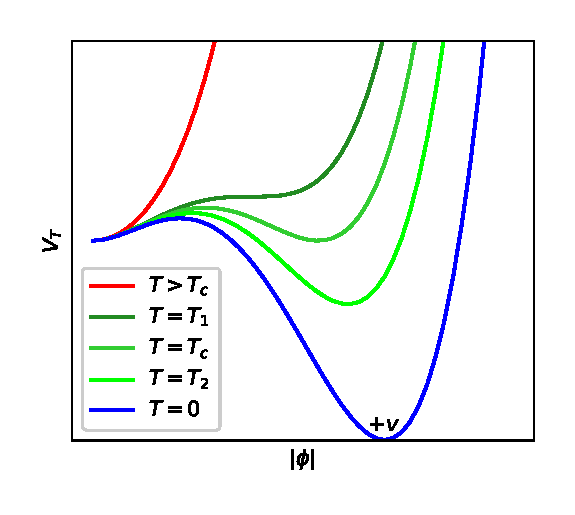
\includegraphics[width=0.6\textwidth]{../pttools/examples/fig/potential.eps}
\caption{The thermal effective potential at different temperatures. Generated with PTtools utilities. See also \cite[fig. 4]{lecture_notes}}
\label{fig:potential}
\end{figure}



For a description on the equation of state, please see the section \ref{general_eq}.

The critical temperature $T_c$ of a phase transition is the temperature where the pressures on both sides of the wall are equal
\begin{equation}
p_+(T_c) = p_-(T_c),
\label{eq:critical_temp}
\end{equation}
where $+$ refers to the symmetric phase in front of the bubble wall,
and the $-$ refers to the broken phase behind the bubble wall.
